\documentclass[a4,12pt]{article}

\usepackage{graphicx}
\usepackage[margin=1in]{geometry}
\usepackage{parskip}
\usepackage{amsmath}
\usepackage{gensymb}
\usepackage{natbib}

\bibliographystyle{agu04}

\title{}
\author{Hans Chen}
\date{}

\begin{document}

Here,
we report on a new ensemble-based dual-state CO2 flux and concentration data assimilation method
developed within the TRACE Regional Atmosphere--Carbon Ensemble (TRACE) framework.
One of the goals of this inversion approach is to enable the assimilation of high volumes of dense satellite observations.
We therefore focus on CO2M,
which will provide substantially more data than existing satellites such as OCO-2.
However,
since the launch of the first CO2M satellite has been delayed,
we used synthetic observations in an OSSE setting instead.
This allows for more in-depth validation of the experiment results as,
unlike in the real world,
the truth in the OSSE is known.
That said,
we emphasize that these results presented here are idealized and do not reflect real-world conditions.


\section{Method}

\begin{figure}[tb]
    \centering
    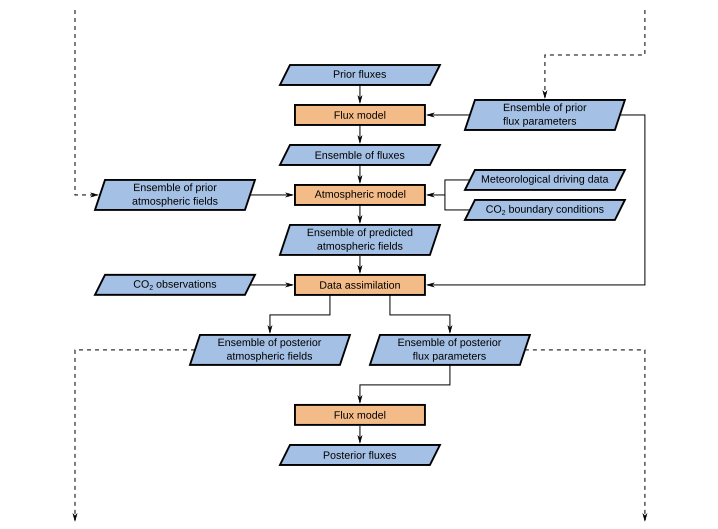
\includegraphics[width=\textwidth]{figures/figure1.png}
    \caption{Data flow from prior to posterior fluxes in the TRACE system.
        Adapted from \citet{chen2023}.
    }
    \label{fig:trace}
\end{figure}

The data assimilation method is based on the ensemble-based simultaneous state and parameter estimation (ESSPE) approach for flux inversion
introduced in \citet{chen2023}.
Figure~\ref{fig:trace} shows a simplified schematic of the approach implemented within the TRACE framework.
TRACE uses different flux models to simulate the fluxes from different sources based on a set of parameters.
In the current implementation,
the parameters are scaling factors applied to prior fluxes,
similar to many other inversion systems,
such as CarbonTracker \citep[e.g.,][]{peters2007}.
In the future it would be possible to implement more sophisticated forward models for fluxes similar to CCFFDAS
(Section 5).

Using a set of perturbed flux parameters,
the system first simulates an ensemble of perturbed prior fluxes.
These fluxes are used as input for a regional atmospheric transport model,
which computes the resulting CO2 concentrations based on the fluxes,
initial conditions,
and lateral boundary conditions.
The initial and lateral boundary conditions can include different CO2 concentrations,
but also different meteorological conditions to simulate atmospheric transport errors \citep{chen2019}.
Unlike most traditional inversion systems,
TRACE uses a full ``online'' mesoscale weather model to downscale meteorological conditions from coarse-resolution data to finer spatial and temporal scales.

In the data assimilation step,
CO2 observations are used to update both the simulated CO2 concentrations and the flux parameters.
This dual-state approach is motivated by the fact that changes in flux parameters propagate to CO2 concentrations through atmospheric transport.
By updating concentrations and parameters simultaneously using ensemble-derived correlations,
the impact of parameter updates is reflected immediately in the concentration state,
eliminating the need to re-run the atmospheric transport model after the parameter update.

Here we provide a summary of the data assimilation approach;
for further details,
we refer to \citet{chen2023}.
The methods implemented in TRACE are based on the ensemble Kalman Filter (EnKF).
In the standard Kalman update,
the background (prior) state vector $\mathbf{x}^b$ is updated based on observations $\mathbf{y}^o$
to yield the analysis (posterior) state vector $\mathbf{x}^a$:
\begin{equation}
    \label{eq:enkf_update}
    \mathbf{x}^a = \mathbf{x}^b + \mathbf{K}(\mathbf{y}^o - \mathbf{H}(\mathbf{x}^b)),
\end{equation}
where $\mathbf{H}$ is the linear observation operator relating model variables to observations,
and $\mathbf{K}$ is the Kalman gain matrix,
computed as:
\begin{equation}
    \label{eq:kalman_gain}
    \mathbf{K} = \mathbf{P}^b \mathbf{H}^\top (\mathbf{H}\mathbf{P}^b \mathbf{H}^\top + \mathbf{R})^{-1}.
\end{equation}
Here,
$\mathbf{P}^b$ is the error covariance matrix for the background (prior) and
$\mathbf{R}$ is the error covariance matrix for the observations.

After assimilating the observations,
the prior error covariance matrix is updated according to:
\begin{equation}
    \label{eq:posterior_cov}
    \mathbf{P}^a = (\mathbf{I} - \mathbf{K}\mathbf{H})\mathbf{P}^b,
\end{equation}
where $\mathbf{P}^a$ is the posterior (analysis) error covariance matrix,
and $\mathbf{I}$ is the identity matrix.

Unlike traditional atmospheric inversion approaches,
which include only fluxes or flux parameters in the state vector,
here $\mathbf{x}$ consists of both gridded two-dimensional flux parameters and three-dimensional CO2 concentrations.
Explicitly propagating the full background error covariance matrix with the dynamical model in such a high-dimensional system is typically computationally prohibitive.
Another computational challenge is to perform the matrix inversion in Equation~\ref{eq:kalman_gain} when the number of assimilated observations is large,
as is often the case for satellite data.
To address these challenges,
the EnKF algorithm approximates the full background error covariance matrix by an ensemble approximation:
\begin{equation}
    \label{eq:ensemble}
    \mathbf{P}^b = \frac{1}{N - 1} \mathbf{X}' \mathbf{X}'^\top,
\end{equation}
where $N$ is the number of ensemble members
and $\mathbf{X}'$ is a matrix whose columns are state vectors of the ensemble perturbations (deviations from the ensemble mean).
Instead of propagating the full $\mathbf{P}^b$,
each ensemble member is propagated forward in time using the dynamical model.

Additionally,
TRACE uses a deterministic square-root formulation of the EnKF,
in which observations are assimilated serially.
Each time an observation is assimilated,
the ensemble mean is updated according to Equation~(\ref{eq:enkf_update}).
At the same time,
the ensemble perturbations are adjusted to reflect the reduced uncertainty after assimilating the observation:
\begin{equation}
    \label{eq:mem_update}
    \mathbf{x}'^a = \mathbf{x}'^b - \widetilde{\mathbf{K}}\mathbf{H}\mathbf{x}'^b,
\end{equation}
where $\mathbf{x}'^a$ and $\mathbf{x}'^b$ are the posterior and prior ensemble perturbations,
respectively,
and $\widetilde{\mathbf{K}}$ is the reduced Kalman gain:
\begin{equation}
    \label{eq:reduced_kalman_gain}
    \widetilde{\mathbf{K}} = \alpha\mathbf{K}, \quad
    \alpha = \left(1 + \sqrt{\frac{\mathbf{R}}{\mathbf{H}\mathbf{P}^b\mathbf{H}^\top + \mathbf{R}}} \right)^{-1}.
\end{equation}

Another advantage of the EnKF implementation is that it allows for the use of the full (potentially nonlinear) observation operator,
which is applied to each ensemble member to map model states to observations.

EnKF applications typically require techniques to address issues such as rank-deficient and spurious correlations in $\mathbf{P}^b$,
as well as filter divergence due to underestimated posterior errors.
Here,
we applied covariance localization,
relaxation to prior perturbations,
and relaxation to initial perturbations for the flux parameters.
See \citet{chen2023} and \citet{houtekamer2016} for detailed information about these techniques.

Atmospheric inversions typically use an assimilation window to account for the time lag for CO2 fluxes to influence CO2 concentrations.
Such a time window is not strictly necessary in the dual-state approach;
the relationship between CO2 fluxes and concentrations are preserved in $\mathbf{P}^b$ between assimilation cycles.
\citet{chen2023} demonstrate that,
even without an assimilation window,
a filtering approach can still constrain fluxes in remote locations
(see their Figure 5).
Including an assimilation window can however be helpful to average out large random errors.
In this deliverable,
we do not use an assimilation window in order to isolate and more clearly assess the impact of each assimilation cycle.


\section{Setup}

We conducted two OSSEs assimilating synthetic XCO2 observations from a hypothetical CO2M satellite
to constrain fluxes in July 2021 (summer) and February 2021 (winter).
We focused on biospheric fluxes,
as they typically generate the strongest regional-scale signals in  atmospheric CO2 concentrations.


\subsection{Data}

We used meteorological initial and boundary conditions from the ERA5 reanalysis \citep{hersbach2020} to drive the regional atmospheric model.
Hourly ERA5 data were obtained at 0.25\degree{} resolution on 37 pressure levels.

For CO2 concentration initial and lateral boundary conditions,
we used the CAMS global inversion-optimized greenhouse gas conditions constrained by surface observations \citep{chevallier2010}.
The CAMS data were provided on a 1\degree{} grid,
interpolated from the hexagon grid ($\sim$90 km resolution) of the transport model.

The prior biospheric fluxes were taken from an LPJ-GUESS simulation (0.5\degree{} resolution) downscaled to hourly values,
see Section 4.2.1 for more details.
Fluxes from the ocean,
fossil fuel emissions, and
fires
were assumed to be perfectly known
and were therefore omitted from the experiments;
their contributions would simply be subtracted out in the data assimilation step.


\subsection{XCO2 observations}

The locations of XCO2 observations were derived from a dataset of simulated CO2M footprints prepared by EUMETSAT for the Copernicus CO2 (CoCO2) project.
The satellite retrievals were averaged to superobservations (superobs) at the same resolution (about 25 km) as the atmospheric transport model.
Only observations over land (nadir mode) were used.
Figure~\ref{fig:xco2} shows the observation count for each model grid cell for the two experiments.

\begin{figure}[tb]
    \centering
    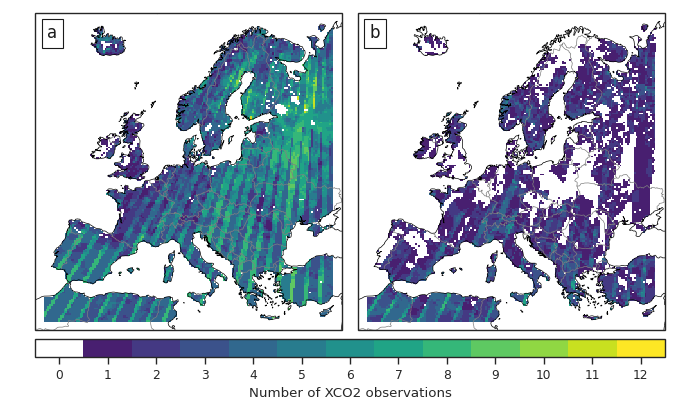
\includegraphics[width=\textwidth]{figures/xco2.png}
    \caption{Number of synthetic XCO2 observations from a hypothetical CO2M satellite in
        that were assimilated in the (a) summer and (b) winter experiments.
        The XCO2 observations were aggregated from their original resolution (about 2 km)
        to superobs with the same resolution as the atmospheric transport model (about 25 km).
    }
    \label{fig:xco2}
\end{figure}

The XCO2 observation values were derived from the reference simulation by calculating the mass-weighted column-averaged CO2 dry-air mole fraction.
To simulate measurement uncertainty,
random errors drawn from a normal distribution with zero mean and standard deviation of 1 ppm were added to all XCO2 observations.
Systematic errors were not included and will be explored in WP5.

For each XCO2 superob,
we calculated the fraction of grid cell covered by observations,
taking also into account cloud cover.
The cloud cover was taken from the reference simulation.
The atmospheric model outputs cloud cover at each vertical level.
To derive the total cloud cover for each grid cell,
we assumed exponential--random overlap between cloud layers,
using a vertical decorrelation length scale of 2 km.
Only superobs in grid cells with over 90\% observation coverage were retained for assimilation.


\subsection{Atmospheric transport model}

TRACE uses the Weather Research and Forecasting (WRF) model coupled with Chemistry (WRF-Chem)
to downscale meteorology and simulate the transport of chemical species.
CO2 was simulated as an inert tracer with no feedback on the meteorological fields.
Here,
the simulations were run at a spatial resolution of 25 km,
60 vertical levels,
and a 1-minute model time step.
The model domain corresponds to the domain shown in Figure~\ref{fig:xco2}.
We refer to \citet{chen2023} for further details about the WRF-Chem configuration.


\subsection{Data assimilation settings}

The inversions were run with 40 ensemble members with perturbed flux parameters.
The flux parameters ($\lambda$) were scaling factors on prior NEE fluxes from LPJ-GUESS:
\[
    NEE_\text{perturbed}(t, x, y) = \lambda(t, x, y) \cdot NEE _\text{prior}(t, x, y)
\]

The flux parameters $\lambda$ were assumed to be constant throughout each one-month experiment.
Furthermore,
errors in $\lambda$ were assumed to have a spatial correlation length of 500 km following a Gaussian decay function.
The prior flux parameter values were set to 1 with an uncertainty (1$\sigma$) of 80\%.

XCO2 observations were assimilated hourly by assigning each observation to its nearest hour.
Observation errors were assumed to be uncorrelated with a magnitude of 4 ppm.
This error is larger than the prescribed random instrument error (1 ppm) to compensate for unrepresented error sources including
systematic biases,
representativeness error,
and atmospheric transport error.
In real applications,
one would likely also apply observation thinning or similar measures to mitigate the impact of spatially correlated observation biases
\citep[e.g.][]{chevallier2007}.
We deliberately used all available observations here to demonstrate that TRACE can feasibly assimilate such dense observational networks.

The impact of each XCO2 observation was localized to a 200 km radius around the measurement location.
To avoid filter divergence,
we applied relaxation to prior perturbations with a relaxation coefficient of 0.2,
and relaxation to initial perturbations with a relaxation coefficient of 0.1.


\subsection{Experiments}

Following standard OSSE practice,
we first ran a reference (``truth'') experiment using a randomly selected set of perturbed flux parameters.
Synthetic XCO2 observations were sampled from this reference simulation and subsequently assimilated in the inversion experiments.

We performed two inversion experiments,
one in July 2021 and another February 2021.
A two-week spin-up period was implemented during which the atmospheric model ran without assimilation,
allowing the model to establish the relationship between flux parameters and atmospheric CO2 concentrations.
Because we used an ensemble Kalman filter,
we optimized only the current parameter values at each assimilation step without retrospectively adjusting past parameter values,
unlike smoothers that optimize over a temporal window.
As a result,
the optimized parameters can appear to exhibit a temporal lag.
To mitigate this lag effect,
we included an additional two-week spin-up period with observation assimilation,
which was excluded when evaluating the monthly fluxes.


\section{Results}

Figure~\ref{fig:rmse} shows the relative error reductions (RERs) in NEE and flux parameters for the summer and winter inversions.
We define RER as one minus the ratio of posterior to prior RMSE.
We used RMSE relative to the truth,
which provides a more realistic metric than posterior uncertainty estimates,
as methods like EnKF tend to underestimate posterior uncertainty.
We present RERs for daily-averaged fluxes and flux parameters to exclude diurnal variations.

\begin{figure}[tb]
    \centering
    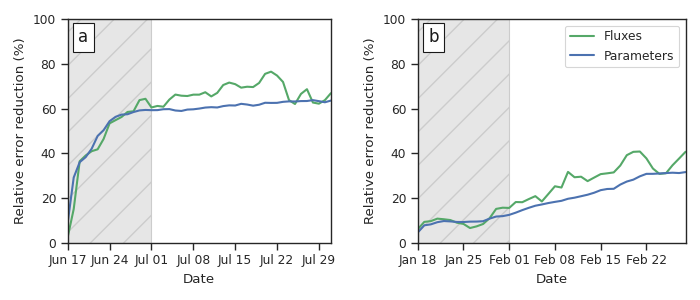
\includegraphics[width=\textwidth]{figures/rmse.png}
    \caption{Relative error reduction in posterior net ecosystem exchange fluxes (green)
        and flux parameters (blue) after assimilating XCO2 observations in
        (a) summer and
        (b) winter 2021.
        The relative error reduction was quantified as one minus the ratio of posterior to prior root-mean-square errors.
        The gray hatched shading indicates the spinup period before the target month.
    }
    \label{fig:rmse}
\end{figure}

By assimilating XCO2 observations,
TRACE is able to substantially reduce the errors in NEE and flux parameters in July 2021,
with a monthly mean RER of 67.3\% and 61.5\%,
respectively.
The RERs differ between fluxes and parameters because in regions with weak fluxes,
the parameter values have little impact on the overall flux and thus remain poorly constrained.
Figure~\ref{fig:rmse}a furthermore shows that the RER increases quickly within the first week and then exhibits a more gradual increase,
suggesting that most of the optimization occurs during the first week of assimilation.

In comparison,
the RERs in February 2021 show slower increases,
reaching relatively lower values of 29.4\% for fluxes and 23.3\% for flux parameters.
This result reflects the effect of reduced satellite coverage in winter (Figure~\ref{fig:xco2}b)
due to large solar zenith angles and increased cloudiness,
combined with weaker biospheric flux signals,
which reduces the covariance between flux parameters and atmospheric CO2 concentrations.
The RERs in Figure~\ref{fig:rmse}b plateau less than in Figure~\ref{fig:rmse}a,
indicating that increased observational coverage would be particularly beneficial in the winter case.

\begin{figure}[tb]
    \centering
    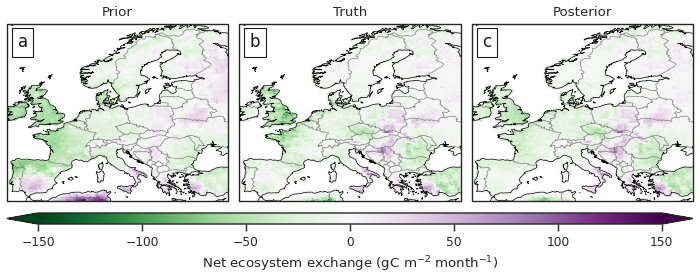
\includegraphics[width=\textwidth]{figures/map_summer.png}
    \caption{Spatial distribution of net ecosystem exchange for
        (a) prior fluxes,
        (b) truth, and
        (c) posterior fluxes
        in July 2021 for the summer experiment.
        The truth was randomly generated and should not be taken as a reflection of reality.
    }
    \label{fig:map_summer}
\end{figure}

Figure~\ref{fig:map_summer} presents the monthly NEE in the summer experiment for the prior, true, and posterior biospheric fluxes.
We reiterate that the ``true'' fluxes are constructed for this OSSE and do not represent real-world conditions.
The inversion is able to bring the posterior fluxes closer to the truth in several regions---%
particularly in northern Africa,
southern Spain,
and parts of Central Europe---%
increasing the spatial correlation with the true fluxes from 0.11 (prior) to 0.87 (posterior).
The error in regional total NEE was reduced from 36.6 TgC month$^{-1}$ in the prior to 3.2 TgC month$^{-1}$ in the posterior,
representing a 91.4\% relative error reduction.
In terms of the RMSE in monthly gridcell-level NEE,
the corresponding relative error reduction was 70.6\%.

\begin{figure}[tb]
    \centering
    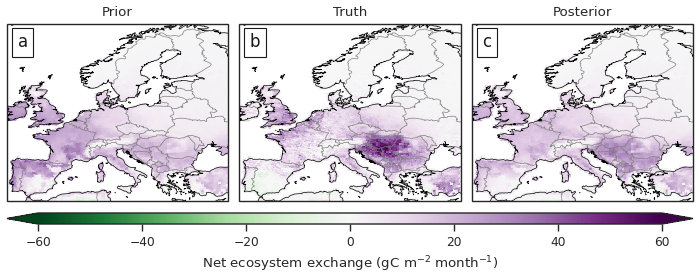
\includegraphics[width=\textwidth]{figures/map_winter.png}
    \caption{Same as Figure~\ref{fig:map_summer} but in February 2021 for the winter experiment.
        Note the different color scale.
    }
    \label{fig:map_winter}
\end{figure}

In the winter experiment,
the adjustments in posterior fluxes are not as pronounced as the summer case (Figure~\ref{fig:map_winter}).
The most noticeable difference from the prior are reduced NEE over parts of Western Europe
and increased NEE over Hungary and the Balkans,
though the latter remains weaker than in the truth.
Spatial correlation increased from 0.57 (prior) to 0.80 (posterior).
The error in regional total NEE was reduced from 7.2 TgC month$^{-1}$ in the prior to 4.6 TgC month$^{-1}$ in the posterior,
a 35.8\% relative error reduction.
The corresponding relative error reduction in monthly gridcell-level NEE was 30.6\%.

To summarize,
these results demonstrate that TRACE's ESSPE approach is promising for assimilating dense satellite observations.
The inversion performance shown here should be interpreted with caution:
error reductions in real applications are likely to be smaller due to additional error sources not represented here.
Nevertheless,
the methods presented provide a pathway to further constrain CO2 fluxes by leveraging increased information from current and future satellite missions.

\bibliography{references}

\end{document}
